\subsection{Dataset}

The original dataset is composed by 4 tables in CSV fomat: \textit{pos.csv}, \textit{rental.csv}, \textit{user.csv}, \textit{device.csv}. This dataset is a subset of another dataset with some sensitive data dropped (like user name or email) and positions manumit in order to protect proprietary data. Although this dataset is only a subset of the proprietary data, the positions amount is really huge and it weighs about 2GB. 

The \textit{pos.csv} table contains all the positions, characterized by latitude, longitude, speed, timestamp and a rental id used to join with \textit{rental.csv} table. The \textit{device.csv} and \textit{user.csv} tables contain the kilometres travelled respectively by a scooter and by a user. At last, the \textit{rental.csv} table contains the start position and end position in couple of longitude and latitude of the rental trajectories with related start and stop timestamps, and the ids used to join the device and user tables. The dataset was subsequently reorganized, filtered and sorted in such a way to have positions in relation with its rental and the positions that belongs in the range of rental start-end time. This operation was really tricky because the total amount of data is huge and I had to optimize database join algorithms and chunks management to be able to handle these data in acceptable time, but in the end the resulting dataset properties diagram is \ref{generated-dataset-diagram}. The figure \ref{fig:starting-point} shows all positions in the two Italy cities contained in \textit{pos.csv} table.

\begin{figure*}[bt]
	\centering
	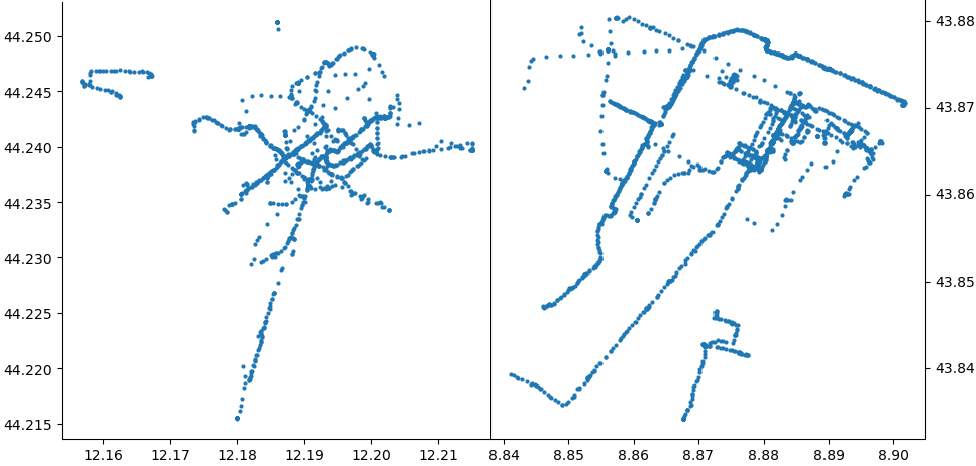
\includegraphics[width=\textwidth]{starting-point}
	\caption{Trajectories without clustering in 2 Italy cities}
	\label{fig:starting-point}
\end{figure*}

Due to how the dataset is constructed, a trajectory can initially be represented as a set of positions $trajectory = \{p_1, p_2, p_3, ..., p_t\}$ that belong to the same rental sorted by the timestamp. Each position $p$ is a tuple $(t_p, lat_p lon_p, s_p)$ where $t_p$ is the server timestamp or the device timestamp, $lat_p$ and $lon_p$ are the longitude and the latitude of the position and $s_p$ is the speed. Formally a trajectory is $trajectory(rental\_id) = \{ p \mid p.rental\_id == rental\_id  \}$ and $TRAJ$ is the set of all trajectories \ref{fig:trajectory-rental}. The resulting figure of the trajectory divided in rental is \ref{fig:rental-plot}.

\begin{figure}[bt]
	\centering
	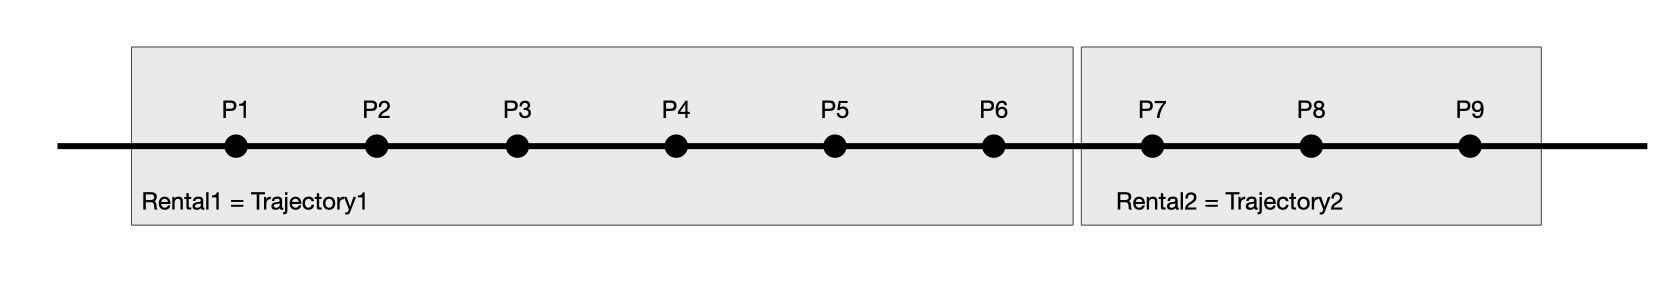
\includegraphics[width=\columnwidth]{trajectory-rental}
	\caption{Trajectories belonging rentals}
	\label{fig:trajectory-rental}
\end{figure}

\begin{figure*}[bt]
	\centering
	\includegraphics[width=\textwidth]{rental-plot}
	\caption{Trajectories belonging rentals}
	\label{fig:rental-plot}
\end{figure*}

\subsection{Heuristics}

After that, I performed some analysis on features. I studied their distribution and I started to think how could be possible to group or divide positions. Two trajectories can be similar in shape and can be divided in time. It means that a sequence of positions, a trajectory, can be similar to another one, evaluating his shape appearance and location in the geographical map, and therefore his sequence of their geographical coordinates. On the other hand, a trajectory can be different to another one if there is a temporal space between each other. 

\begin{table}
	\centering
	\caption{Number of features and samples of generated dataset}
	\begin{tabular}{ l r r }
		\hline
		Dataset & Samples & Features \\ \hline
		rental & 14826 & 10 \\ 
		pos & 817076 & 18 \\ 
		merge & 817076 & 18 \\
		dataset & 14826 & 13 \\
		partition city 1 & 608251 & 18 \\
		partition city 2 & 202795 & 18 \\ \hline
	\end{tabular}
\end{table}

As result I implemented 3 different clustering heuristics performed in a systematic and statistical way on the entire sequence of positions:
\begin{itemize}
	\item \textbf{timedelta heuristic}: considers that a trajectory of a rental can be divided in a sequence of trajectories if the time gap between a position and previous one exceeds a \textit{timedelta} value. First of all I calculated the time gaps for each set of positions grouping in rental: 
	\begin{align}
		TIMEGAPS = \{t.time - shift(t, -1).time \mid \forall t \in TRAJ \}
	\end{align}
	where \verb|shift(t, -1)| shifts the trajectory backward and the field \verb|.time| gives the timestamp of each position in trajectory. The \textit{timedelta} value has been manually assigned or automatically calculated with the statistical empirical rule (three-sigma rule or 68-95-99.7 rule). The timegaps set is then used to divide the trajectories if the gap exceeds the defined timedelta (figure \ref{fig:trajectory-timedelta}).
	
	\begin{figure}[bt]
		\centering
		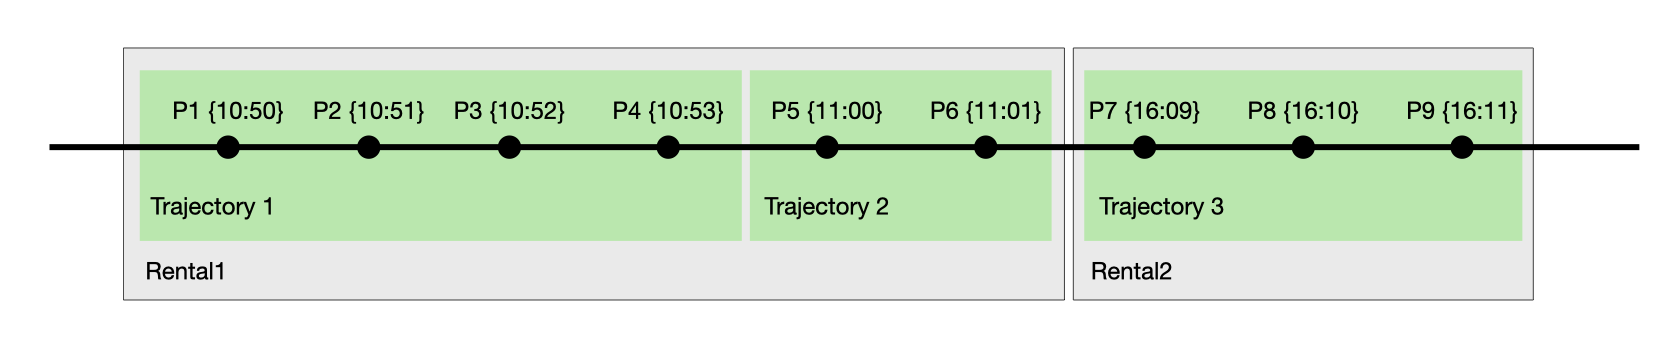
\includegraphics[width=\columnwidth]{trajectory-timedelta}
		\caption{Trajectories belonging timedelta heuristic}
		\label{fig:trajectory-timedelta}
	\end{figure}
	
	\item \textbf{spreaddelta heuristic}: considers that a rental trajectory can be considered similar to another one if they spread a similar amount of area (figure \ref{fig:spreaddelta-pred}). I calculate the spread area for each rental trajectory in the following way: 
	\begin{align}
		SPREADS = \{max(t) - min(t) \mid \forall t \in TRAJ \}
	\end{align}
	where \verb|max(t)| and \verb|min(t)| calculate respectively the maximum and the minimum latitude and longitude of a set of positions, and \verb|TRAJ| is the set of trajectories that can be grouped for each rental or for the \textit{timedelta heuristic} (figure \ref{}). Also in this case, I exploited the empirical rule to compute the spreaddelta value. 
	
	\begin{figure}[bt]
		\centering
		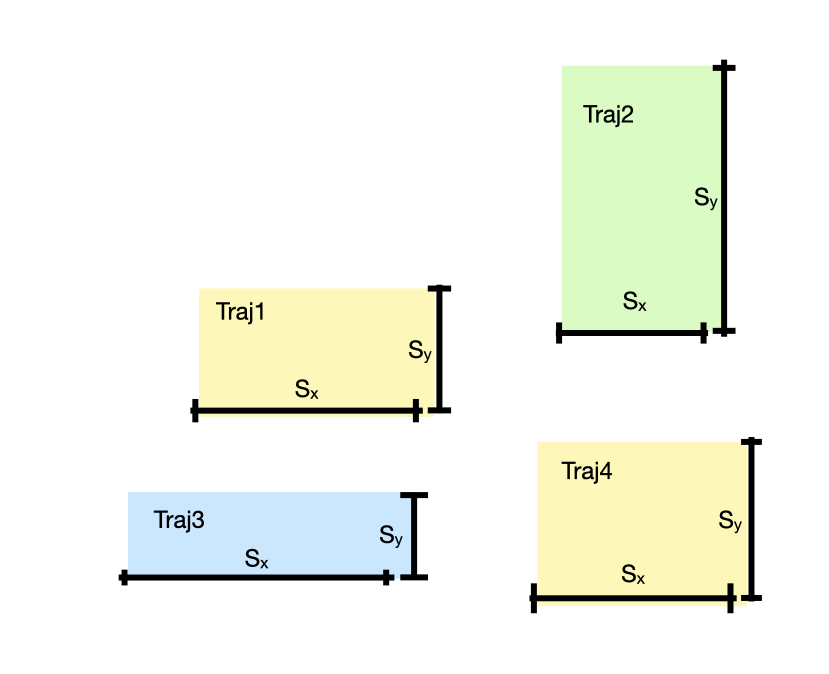
\includegraphics[width=\columnwidth]{spreaddelta-pred}
		\caption{For spreaddelta heuristic $Traj1$ and $Traj4$ are similar because they spread a similar amount of area}
		\label{fig:spreaddelta-pred}
	\end{figure}

	\begin{figure}[bt]
		\centering
		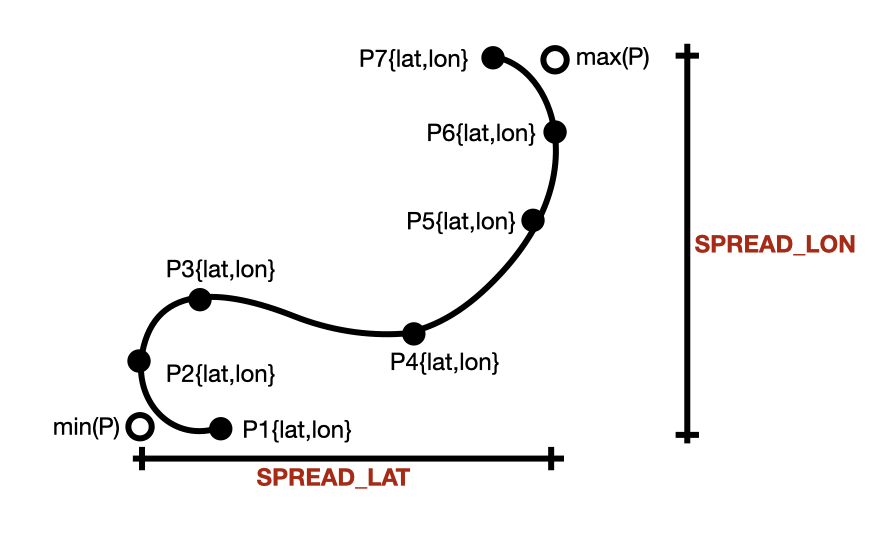
\includegraphics[width=\columnwidth]{spreaddelta-calc}
		\caption{Spreads calculus in trajectory}
		\label{fig:spreaddelta-calc}
	\end{figure}
	
	\item \textbf{edgedelta heuristic}: acts as the \textit{spreaddelta heuristic}, but it considers the edges of a trajectory, or rather the first position and the last position of a trajectory \ref{fig:edgedelta-pred}. The main problem here is that the distribution of edge positions has 2 centres or, in other words, it is bimodal. To resolve this issue I applied for simplicity only 1 iteration of \textit{Mean Shift} starting from a random position in order to get closer to one of 2 centre. The set of edges is calculated in the following way (figure \ref{fig:edgedelta-calc}): 
	\begin{align}
		EDGES = \{concat(p[0], p[-1]) \mid \forall t \in TRAJ \}
	\end{align}
	
	\begin{figure}[bt]
		\centering
		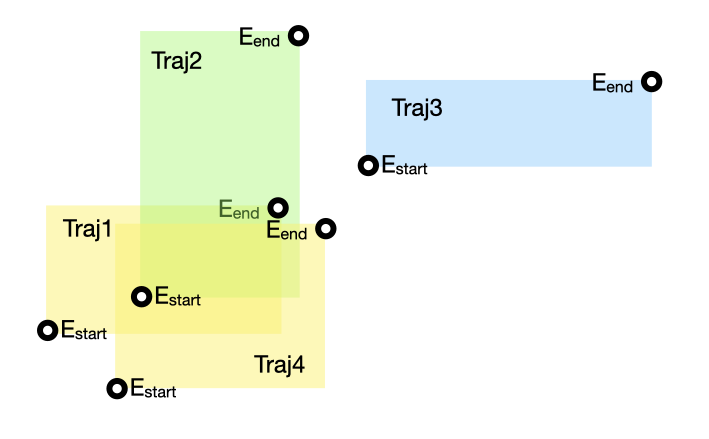
\includegraphics[width=\columnwidth]{edgedelta-pred}
		\caption{For edgedelta heuristic $Traj1$ and $Traj4$ are similar because they start and finish nearly}
		\label{fig:edgedelta-pred}
	\end{figure}
	
	\begin{figure}[bt]
		\centering
		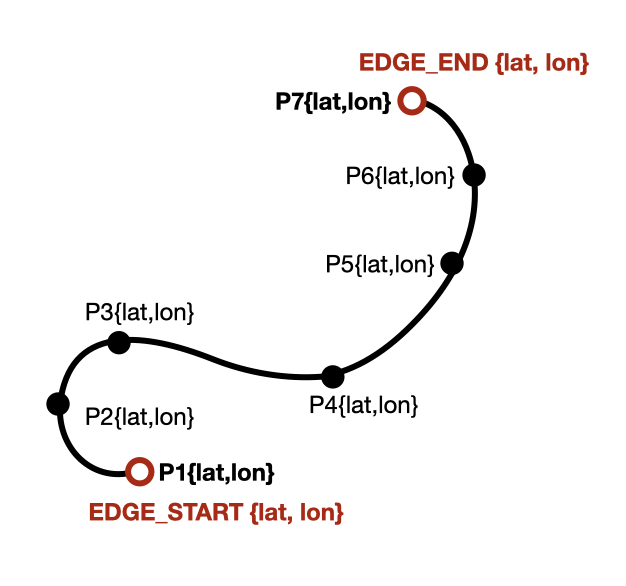
\includegraphics[width=\columnwidth]{edgedelta-calc}
		\caption{Edges calculus in trajectory}
		\label{fig:edgedelta-calc}
	\end{figure}

	\item \textbf{coorddelta heuristic}: it is a combination of spread and edge heuristics in order to combine the main advantages of each other. 
\end{itemize}

\subsection{Feature extraction}

For feature extraction I decided to perform \textit{Standardization}, \textit{Normalization} and than \textit{Principal Component Analysis (PCA)}.

As feature extraction, I considered that the work done for the heuristic algorithms could return useful for clustering algorithms. In particular $TIMEGAPS$, $SPREADS$ and $EDGES$ sets can be used as new features for my data. Therefore, I integrate my data features with the heuristic values and I run the pipeline of \textit{Standardization}, \textit{Normalization}, \textit{PCA} and than clustering algorithms. In particular, I tried to perform this pipeline with space and time features together, with only space features, and then with space and heuristic features together. Moreover I tried to perform clustering algorithm on the whole trajectories and even on one city at a time.

The feature extraction algorithm for Deep Clustering is the behavior feature extraction. The key idea of the behavior feature extraction is to utilize a sliding window to traverse the records and extract features in each window. As shown in \ref{fig:moving-behavior-feature}, with a sliding window, we aim to obtain space- and time- invariant features to describe the moving behaviors of the object.

\begin{figure}[bt]
	\centering
	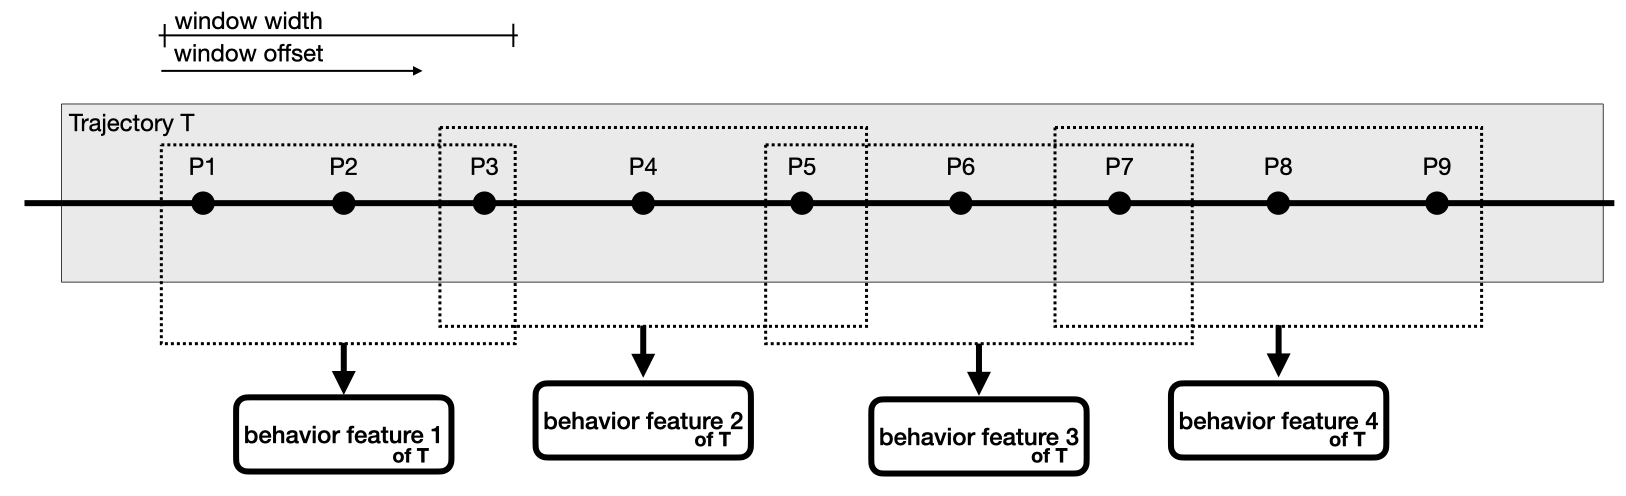
\includegraphics[width=\columnwidth]{moving-behavior-feature}
	\caption{Moving behavior feature extraction algorithm}
	\label{fig:moving-behavior-feature}
\end{figure}

Let $L$ and $offset$ denote the width and the offset of the sliding window, respectively. While classic methods often choose $offset = L$, a finer granularity of $offset= 1/2 * L$ can effectively lead to better performance. 
The moving behavior changes can be reflected by the differences of the attributes between two consecutive records. Let us consider a window with $L$ records. The records in this window are denoted as $W = (p_1, p_2, ..., p_i, ..., p_L)$. 
Assume the attributes in each record consist of speed and rate of turn (ROT). The extracted attributes for the moving behaviors include: time interval $\Delta t_i = t_{p_i} - t_{p_{i-1}}$, change of position $\Delta lat_i = lat_{p_i} - lat_{p_{i-1}}$ and $\Delta lon_i = lon_{p_i} - lon_{p_{i-1}}$, change of speed $\Delta s_i = s_{p_i} - s_{p_{i-1}}$ and change of ROT $\Delta r_i = r_{p_i} - r_{p_{i-1}}$, where $i$ ranges from 2 to $L$. 

In this way, a window with $L$ records has $L-1$ moving behavior attributes of kind $(\Delta lat, \Delta lon, \Delta s, \Delta r)$.
If $L => 1$, for each $i$ from 1 to $L-1$, we compute $\Delta t_i$, $\Delta lat_i$, $\Delta lon_i$, $\Delta s_i$ and $\Delta r_i$. Further compute the change rate of these features $f_i = (f_{\Delta lat_i}, f_{\Delta lon_i}, f_{\Delta s_i}, f_{\Delta r_i})$ in which $f_{\Delta lat_i} = \Delta lat_i / \Delta t_i$, $f_{\Delta lon_i} = \Delta lon_i / \Delta t_i$, $f_{\Delta s_i} = \Delta s_i$, $f_{\Delta r_i} = \Delta r_i$. For two consecutive records, $f_{\Delta lat_i}$ and $f_{\Delta lon_i}$ stand for the average speed, $f_{\Delta s_i}$ stands for the change of speeds and $f_{\Delta r_i}$ stands for the change of ROTs. After computing these features in each pair, we get a feature set $f = {f1, f2, ..., f_{L-1}}$. We use the statistic of f to generate the features in the sliding window. Here, six statistics ${mean, max, 75\%quantile, 50\%quantile, 25\%quantile, min}$.

In summary, the moving behavior features of each window has $4 * 6 = 24$ dimensions that consist of ${f_{\Delta lat}, f_{\Delta lon}, f_{\Delta s}, f_{\Delta r}} \times {mean, max, 75\%quantile, 50\%quantile, 25\%quantile, min}$.
If $R = 0$,  skip this window. Algorithm 1 shows the generation procedure of moving behavior feature sequence.
For each trajectory in $T$, we generate the moving behavior sequence for it. Then, we put these sequences in a set and denote it as $BS = {BTR1,BTR2,...,BTRN}$. Finally, we normalize each feature to prepare for the next sequence to sequence auto-encoder layer.

\subsection{Clustering}

The clustering algorithms that I used are the following: 
\begin{itemize}
	\item \textit{K-Means}: choose centroids that minimise the \textit{inertia}, or \textit{within cluster sum of squares (WCSS)} criterion.
	\item \textit{Mean Shift}: discover blobs in a smooth density of samples with the purpose to find the mean of points within a given region. 
	\item \textit{Gaussian Mixture}: implements the \textit{expectation-maximization (EM)} algorithm for fitting mixture of Gaussian models. 
	\item \textit{Full and Ward Hierarchy Agglomerative}: hierarchical clustering using a bottom up approach and minimizes the maximum distance between observations in pairs of clusters (Full) or minimizes the sum of squared differences between all clusters (Ward). 
\end{itemize}

\subsection{Deep Clustering}

An autoencoder is a type of deep neural network used to learn efficient codings of unlabeled data (unsupervised learning). The encoding is validated and refined by attempting to regenerate the input from the encoding. The autoencoder learns a representation (encoding) for a set of data, typically for dimensionality reduction, by training the network to ignore insignificant data (Figure \ref{fig:autoencoder-schema}). 

\begin{figure}[bt]
	\centering
	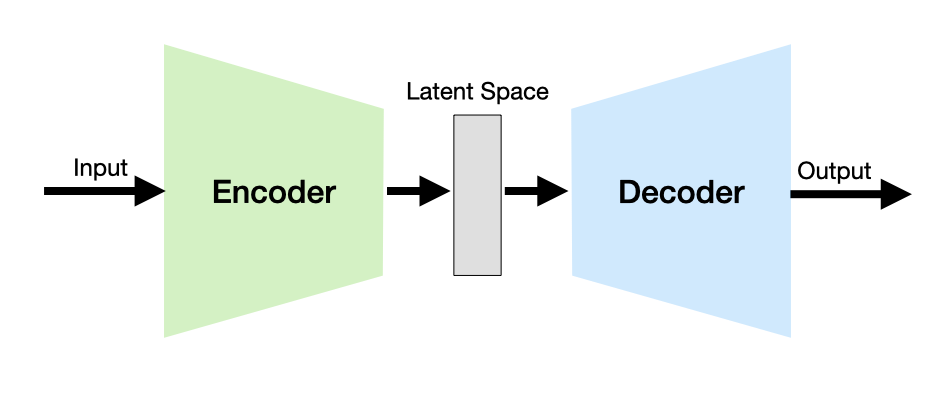
\includegraphics[width=\columnwidth]{autoencoder-schema}
	\caption{Autoencoder main principle}
	\label{fig:autoencoder-schema}
\end{figure}

The LSTM autoencoder models used are the following:
\begin{itemize}
	\item \textit{Simple Autoencoder}: the model is composed by an LSTM that which acts as encoder and another LSTM that acts as decoder. Initially the state of the encoder LSTM is randomly initialized. During training process, the output generated from the encoder is passed to the decoder and the LSTM decoder state is initialized with the encoder one (figure \ref{fig:lstm-autoencoder-schema}). 
	
	\begin{figure}[bt]
		\centering
		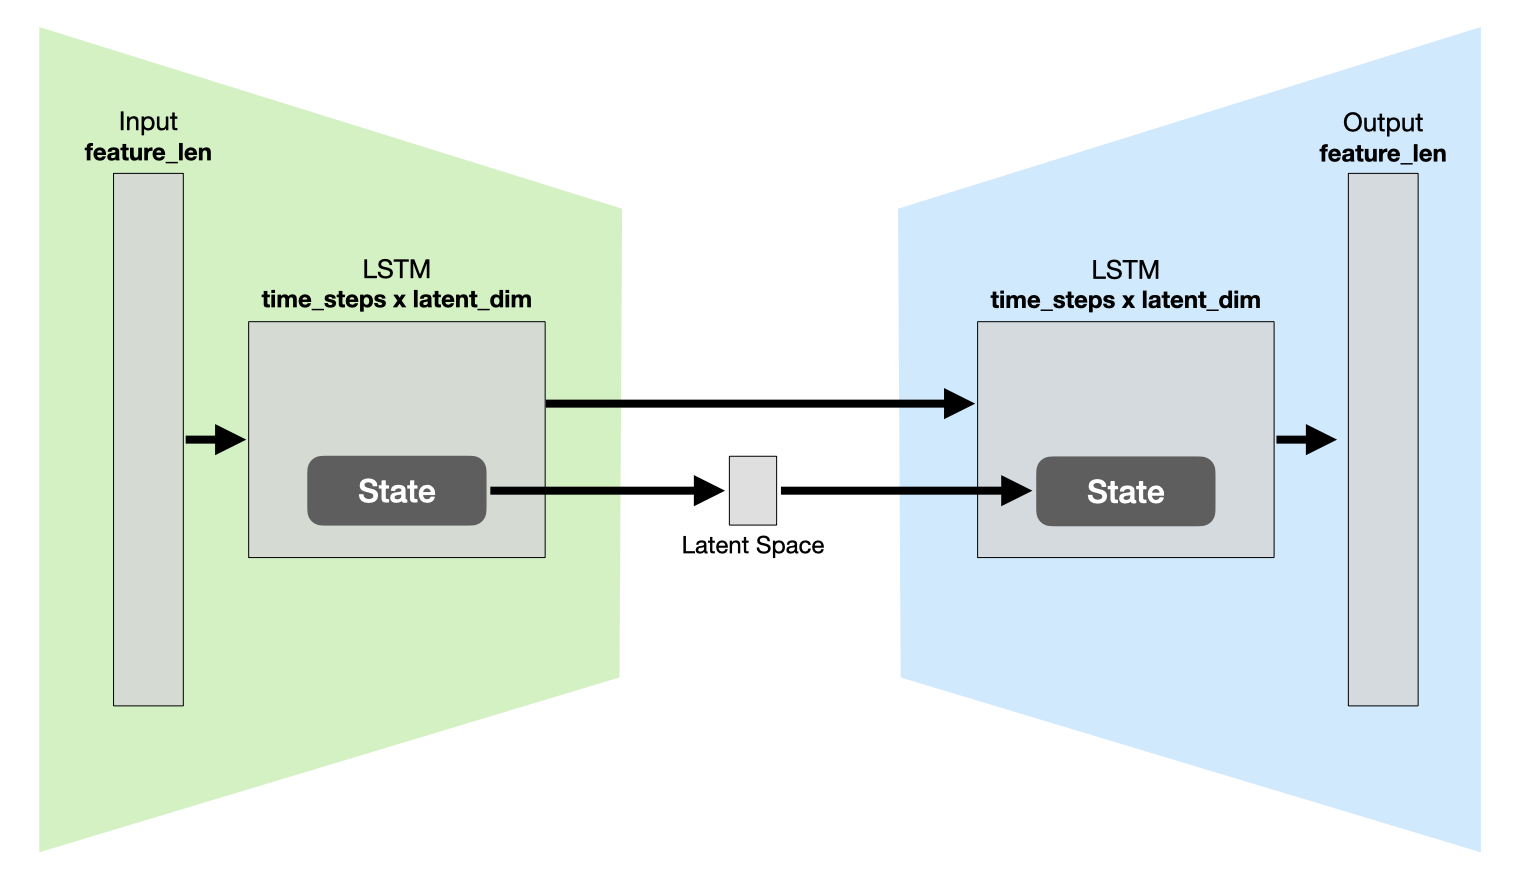
\includegraphics[width=\columnwidth]{lstm-autoencoder-schema}
		\caption{Simple Autoencoder schema}
		\label{fig:lstm-autoencoder-schema}
	\end{figure}

	\item \textit{Autoregressive Autoencoder}: the encoder LSTM reads the input sequence sequentially and the hidden state $state_i$ is updated accordingly. After the last position of the trajectory is processed, the hidden state $state_t$ is used as the representation for the whole sequence. Then, the decoder first generates the output by taking $state_t$ as the initialized hidden state of the decoder LSTM and the last output of the encoder as the first input of the decoder, and then further generate the other output taking as input the previous output, so as to form the following autoregressive model \ref{fig:autoregressive-autoencoder-schema}.
	\item \textit{Addons Autoencoder}: the model is the same of the previous one, but the decoder part is substitute with an already implemented decoder contained in \textit{TensorFlow Addons} library. The decoder is named \texttt{BasicDecoder} and it is trained with the \texttt{TrainingSampler} that reads output distribution of the current decoding step and pass it to the next decoding step (figure \ref{fig:autoregressive-autoencoder-schema}).
	
	\begin{figure}[bt]
		\centering
		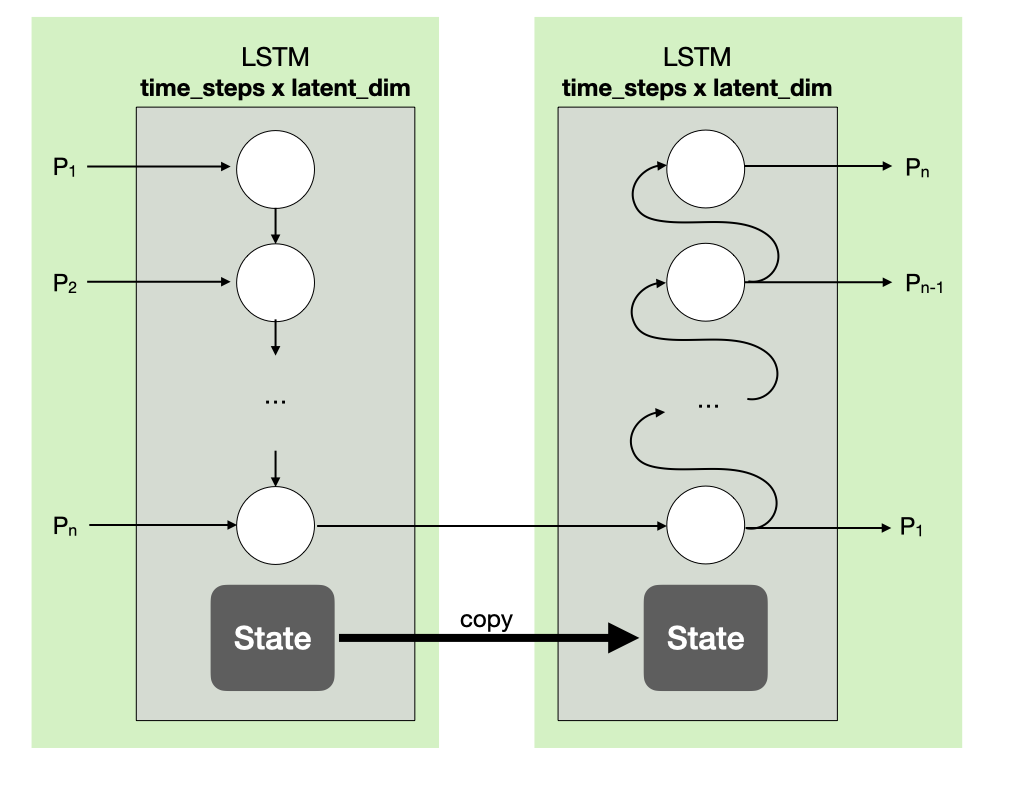
\includegraphics[width=\columnwidth]{autoregressive-autoencoder-schema}
		\caption{Autoregressive Autoencoder schema}
		\label{fig:autoregressive-autoencoder-schema}
	\end{figure}
\end{itemize}

The target of the decoder is to reconstruct the input sequence. In other words, the encoder LSTM and decoder LSTM are trained together by minimizing the reconstruction error. 

The input target of the LSTM autoencoder models could be the moving behavior features but also the raw positions features. In fact, a fundamental characteristic of the neural networks is to learn well the trend of the training inputs, consequently in this case it is not essential to apply a feature transformation algorithm when there are already many. 

In order to reproduce the sliding window behavior when raw positions are used, the training is performed creating a dataset of sliding windows over the input timeseries trajectory. Then, the input shape for the autoencoder becomes $batch_size \times number_of_sliding_window \times sliding_window_width $.